\section{05.11.2025}{2-formy}

$E$ - przestrzeń liniowa, 
$$\bigwedge^2E^*=\{B:E\times E\to \R\;:\;\text{dwuliniowe, }B(e,f)=-B(f,e)\}$$
Kiedy $\dim(E)=2$ to $\dim(\bigwedge^2E^*)=1$.

Dla $\alpha, \beta\in E^*$ definiujemy $\alpha\wedge\beta\in\bigwedge^2E^*$
$$(\alpha\wedge\beta)(e,f)=\alpha(e)\beta(f)-\alpha(f)\beta(e)$$

Jeśli $E=T_p\Sigma$ to $E^*=T^*_p\Sigma$ i $\bigwedge^2T^*_p\Sigma=\bigwedge^2E^*$
dla współrzędnych $(x,y)$ mamy $dx,dy\in T_p^*\Sigma$ i
$$dx\wedge dy\in\bigwedge^2T_p^*\Sigma$$
jest bazą

gładka $2$-forma $\omega$ na $\Sigma$ to
$$\omega:\Sigma\to \bigwedge^2T^*\Sigma=\bigcup_{p\in\Sigma}\bigwedge^2T_p^*\Sigma$$
$$\omega(p)\in\bigwedge^2T_p^*\Sigma$$
lokalnie we współrzędnych 
$$\omega=f(x,y)dx\wedge dy=f(x,y)dxdy$$
[$\omega(p)=f(x(p), y(p))[dx]_p\wedge[dy]_p$]

Jak wygląda zmiana współrzędnych $(x,y)\to(x', y')$?
$$f(x(x', y'), y(x', y'))(\frac{\partial x}{\partial x'}dx'+\frac{\partial x}{\partial y'}dy')\wedge(\frac{\partial y}{\partial x'}dx+\frac{\partial y}{\partial y'}dy)=f(x(x',y'),y(x'y'))(\frac{\partial x}{\partial x'}\frac{\partial y}{\partial y'}-\frac{\partial x}{\partial y'}\frac{\partial y}{\partial x'})dx\wedge dy$$

\subsection{Całka}

Jeśli $\supp(\omega)\subseteq U$, gdzie $U$ jest zbiorem mapowym współrzędnych $(x, y)$ to 
$$\int_\Sigma\omega=\int_U\omega=\int_Uf(x,y)dxdy$$
to nie zależy od wyboru współrzędnych na nośniku $\omega$.

Ogólnie jeśli mamy $\omega$ o zwartym nośniku, $\omega\in\Omega_c^2(\Sigma)$, to możemy ten nośnik pokryć zbiorami mapowymi $\supp(\omega)\subseteq \bigcup_{i\leq n}U_i$. Rozkład jedności: $\chi_i\in C_c^\infty(U_i)$ takie, że $\sum \chi_i=1$.
$$\int_\Sigma\omega=\sum_i\int_{U_i}\chi_i\omega$$

\begin{definition}{różniczka}{}
  $$d:\Omega^1(\Sigma)\to \Omega^2(\Sigma)$$
  \begin{enumerate}
    \item $\alpha_1=\alpha_2\implies d\alpha_1=d\alpha_2$ na $U$
    \item $ddf=0$ dla $f\in C^\infty(\Sigma)=\Omega^0(\Sigma)$
    \item $d(f\alpha)=df\wedge \alpha+fd\alpha$
  \end{enumerate}
  lokalnie dla $\Omega^1(\Sigma)\ni \alpha=fdx+gdy$:
  $$d\alpha=d(fdx)+d(gdy)=df\wedge dx+fddx+dg\wedge dy+gddy=(f_xdx+f_ydy)\wedge dx+...$$
\end{definition}

\begin{theorem}{stokes}{}
  $\Sigma$ - powierzchnia z brzegiem, $\alpha\in\Omega_c^1(\Sigma)$
  wtedy
  $$\int_{\partial \Sigma}\alpha=\int_\Sigma d\alpha$$
\end{theorem}

\begin{proof}
  rozkład jedności + rachunek w mapie
\end{proof}

Zadanie: $f,g\in C^\infty\R^2$ czy istnieje $F\in C^\infty(\R^2)$ takie, że $F_x=f$, $F_y=g$?

jest na to konieczny warunek, bo $F_{xy}=f_y$, $F_{yx}=g_x$ a dla gładkich funkcji $F_{xy}=F_{yx}$.

innymi słowy pytamy czy istnieje $F$ takie, że $$dF=fdx+gdy=\alpha$$

TAK $\iff d\alpha=0$.

$\implies d\alpha=ddF=0$

$\impliedby$ krzywa $\gamma$ idzie od $(0,0)$ do $(0,y)$ i potem do $(x,y)$ ({\color{red}rysunek}) $F(x,y)=\int_{\gamma}\alpha=\int_0^xg(0,t)dt+\int_0^xf(t,y)dt$
co jeśli jest $\overline{F}$ (całka po krzywej $\xi$ $(0,0)-(x,0)-(x,y)$)? 
$$F-\overline{F}=\int_\gamma\alpha-\int_\xi\alpha=\int_{\gamma\cup-\xi}\alpha=\int_{\square}d\alpha=0$$
można się przyczepić, że kwadrat nie ma gładkiego brzegu, ale jak go ugładzimy to wyjdzie to samo i to nam nie przeszkadza

policzyliśmy właśnie, że $H^1(\R^2)=0$

\subsection{Kohomologie de Rhama}

$$\begin{tikzcd}
  \Omega^0(\Sigma)\arrow[r, "d^0"] & \Omega^1(\Sigma)\arrow[r, "d^1"] & \Omega^2(\Sigma)
\end{tikzcd}$$

$H^0(\Sigma)=\ker d^0$
$H^1(\Sigma)=\ker d^1/\im d^0$
$H^2(\Sigma)=\Omega^2(\Sigma)/\im d^1$
wpierw będziemy się skupiać na $H^1$

\begin{fact}{}{}
  \begin{enumerate}
    \item $H^1(\R^2)=0$
    \item $H^0(\Sigma)=\R^n$, gdzie $n$ to liczba składowych spójnych $\Sigma$
  \end{enumerate}
\end{fact}

\begin{example}[m]
  \item annulus $A$

    \begin{center}
      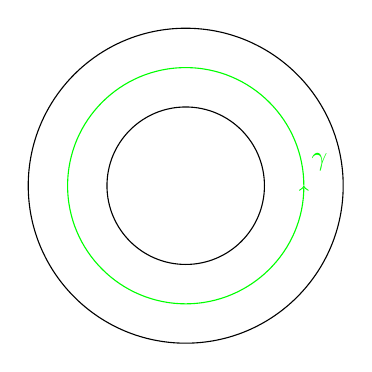
\begin{tikzpicture}
        \draw (0,0) circle (1);
        \draw (0,0) circle (2);

        \draw[->, green] (1.5, 0) arc (0:360:1.5);
        \node at (1.7, .3) {\color{green}$\gamma$};
      \end{tikzpicture}
    \end{center}
    $H^1(A)\neq 0$, $d\theta\in \Omega^1(A)$, $dd\theta=0$ dla $d\theta\in \ker(d^1)$
    $$\int_\gamma d\theta=\theta(\gamma(1))-\theta(\gamma(0))=2\pi$$
    gdyby $d\theta=dF$ dla $F\in C^\infty$ to wówczas $\int_\gamma d\theta=\int_\gamma dF=F(\gamma(1))-F(\gamma(0))=0$

  \item sfera $S^2$ (mapy: biegun płn $U$ i płd $V$)

    Niech $\alpha\in\Omega^1(S^2)$, $d\alpha=0$, $d|_U=df_U$, $\alpha|_V=df_V$

    patrzymy jak $f_U- f_V=$ się zachowuje na przekroju $U\cap V$
    $$d(f_U-fV)=d\alpha-d\alpha=0\implies f_U-f_V=c$$
    
    dla $\Omega^0(S^2)\ni f=f_U\cup (f_V+c)$, $df=\alpha$
    
    czyli $H^1(S^2)=0$
  \item torus $T^2=S^1\times S^1$ myślimy o nim jak o dwóch współrzędnych kątowych $\theta$ i $\phi$
    \begin{center}
      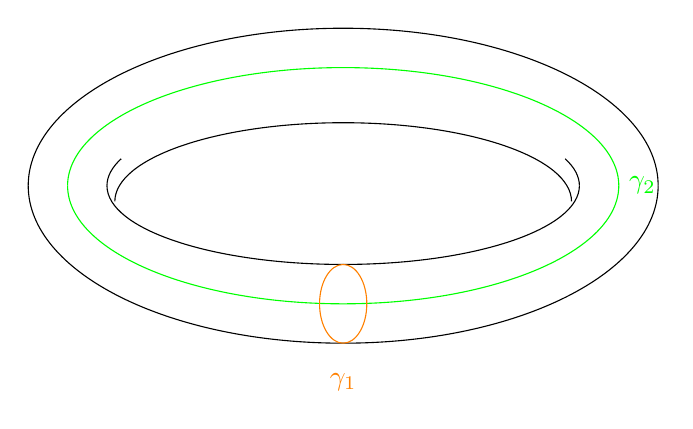
\begin{tikzpicture}
        \draw (0,0) arc (0:-180:4 and 2);
        \draw (0,0) arc (0:180:4 and 2);
        \draw (-1, 0) arc (0:-180:3 and 1);
        \draw (-1, 0) arc (0: 20: 3 and 1);
        \draw (-7, 0) arc (-180:-200: 3 and 1);
        \draw (-1.1, -.2) arc (0:180: 2.9 and 1);

        \draw[green] (-.5, 0) arc (0:-180:3.5 and 1.5);
        \draw[green] (-.5, 0) arc (0:180:3.5 and 1.5);
        \node at (-.2, 0) {\color{green}$\gamma_2$}; 

        \draw[orange] (-4, -2) arc (-90:90:.3 and .5);
        \draw[orange] (-4, -2) arc (-90:-270:.3 and .5);
        \node at (-4, -2.5) {\color{orange}$\gamma_1$};
      \end{tikzpicture}
    \end{center}
    $$\begin{tikzcd}
      \iota:H^1(T)\arrow[r] & \R^2\\ 
      \alpha\arrow[u, phantom, sloped, "\in"] \arrow[r] & (\int_{\gamma_1}\alpha, \int_{\gamma_2}\alpha)\arrow[u, phantom, sloped, "\in"]
    \end{tikzcd}$$
    $\iota$ jest dobrze określona, bo
    $$\iota(df)=(\int_{\gamma_1}df, \int_{\gamma_2}df)=(0,0)$$
    $\iota$ jest epimorfizmem, bo $\iota(d\theta)=(1,0)$ i $\iota(d\phi)=(0,1)$
    $\iota$ jest monomorfizmem, bo jeśli $d\alpha=0$ to $\int_{\gamma_1}\alpha=\int_{\gamma_2}\alpha=0$. Niech $\alpha=Pd\theta+Qd\theta$
    $$0=\int_{\gamma_1}\alpha=\int_0^{2\pi}P(\theta, \phi)d\theta$$
    dla $\phi\in\R$
    $$f(\theta, \phi)=\int_0^\theta P(\xi, \phi)d\xi$$
    $f_\theta=P$
    popatrzymy na zmodyfikowane $\alpha$, 
    $$\overline{\alpha}=\alpha-df=\overline{Q}d\phi$$
    $$0\int_{\gamma_2}\overline{\alpha}=\int_0^{2\pi}\overline{Q}(\theta, \xi)d\xi$$
    czyli $g(\theta, \phi)=\int_0^\phi\overline{Q}(\theta, \xi)d\xi$ czyli $g_\phi=\overline{Q}$

    ZDJECIE

\end{example}

ćwiczenia: policzyć $H^1$ dla
\begin{itemize}
  \item $S^1\times \R$
  \item powierzchni genusu 2
  \item powierzchni genusu $g$
\end{itemize}


\subsection{kohomologie de Rhama o zwartym nośniku}

$\Sigma$ bez brzegu (zorientowana bo Riemanna)

$H^*_c(\Sigma$ kohomologie de Rhama o zwartym nośniku
zamiast $\Omega^*$ używamy $\Omega_c^*$

$$\int_\Sigma:H^2_c(\Sigma)\to \R$$

\begin{fact}{}{}
  odwzorowanie wyżej jest izomorfizmem
  
  ($\Sigma$ spójna, zorientowana, bez brzegu)
\end{fact}

\begin{proof}
  $\int_\Sigma$ jest na

  różnowartościowość:

  $$\Sigma=\R^2$$
  niech $\omega\in\Omega_c^2(\R^2)$, $\int_{\R^2}\omega=0$

  $\omega=R(x,y)dxdy$, $R\inC_c^\infty(\R^2)$

  $r(x)=\int_{-\infty}^\infty R(x,y)dy$
  $\psi$ to pomocnicza bump funkcja ($\int_\R \psi(t)dt=1$)

  $\overline{R}(x,y)=R(x,y)=r(x)\psi(y)$
  $$\int_\R\overline{R}(x,y)dy=0$$
  $$P(x,y)=\int_{-\infty}^y(\overine{R}(x,t)dt$$
  $P\inC_c^\infty(\R^2)$, $P_y=\overline{R}$

  $$Q(x,y)=\psi(y)\int_{-\infty}^xr(t)dt$$
  $Q\in\Omega_c^\infty(\R^2)$, $Q_x(x,y)=\psi(y)r(x)$

  $$R(x,y)=\overline{R}(x,y)+r(x)\psi(y)=P_y+Q_x$$
  $$\omega=d(-Pdx+Qdy)$$


  Niech $\Sigma$ dowolna,
  $\supp \omega\subseteq K$ zwarty $\subseteq U_1\cup U_2\cup...\cup U_n$ mapowe
  
  zrobimy indukcję względem $n$

  $U=U_1$, $V=U_2\cup...\cup U_n$

  dobieramy $f$, $g$ tak, że $f\in C_c^\infty(U)$, $g\in C_c^\infty(V)$, $f+g=1$ na $K$

  $I=\int_\Sigma f\omega=-\int_\Sigma g\omega$

  weźmy $\tau\in \Omega_c^2(U\cap V)$, $\int_\Sigma \tau=1$

  $f\omega-I\tau=d\alpha$ w $U$
  
  $g\omega+I\tau=d\beta$ w $V$

  $\omega=f\omega+g\omega=d\alpha+d\beta$


\end{proof}

Niech $\gamma$ będzie pętlą w $\Sigma$, wtedy $I_\gamma:H^1(\Sigma)\to\R$, $\alpha\mapsto\int_\gamma\alpha$

$\theta\in\Omega_c^1(\Sigma)$, $d\theta=0$ to $J_\theta:H^1(\Sigma)\to \R$, $\Sigma$ bez brzegu,
$$\alpha\mapsto \int_\Sigma\theta\wedge\alpha=\int-d(f\theta)=\int_{\partial \Sigma}f\theta=0$$

\begin{theorem}{}{}
  $\forall\;\gamma\;\exists\;\theta\;I_\gamma=J_\theta$
\end{theorem}

\begin{proof}
  rozcinam krzywą zbiorami mapowymi
  na każdym przecięciu dwóch zbiorów mapowych (poza pierwszym) wybieram dyszczek $D_i$

  dobieram $\omega_i\in\Omega_c^2(D_i)$, $\int_{D_i}\omega_i=1$

  $$\omega_{i+1}-\omega_i\in\Omega_c^2(U_i)$$
  całka po tym jest zero, więc $\omega_{i+1}-\omega_i=d\theta_i$, $\theta_i\in\Omega_c^1(U_i)$
  $$\theta=\sum\theta_i$$
  $d\theta=\sum d\theta_i=\sum(\omega_{i+1}-\omega_i)=0$

  pozostaje $J_\theta=I_\gamma$
  ORBAZEK
\end{proof}


